%% Copernicus Publications Manuscript Preparation Template for LaTeX Submissions
%% ---------------------------------
%% This template should be used for copernicus.cls
%% The class file and some style files are bundled in the Copernicus Latex Package, which can be downloaded from the different journal webpages.
%% For further assistance please contact Copernicus Publications at: production@copernicus.org
%% https://publications.copernicus.org/for_authors/manuscript_preparation.html


%% Please use the following documentclass and journal abbreviations for preprints and final revised papers.

%% 2-column papers and preprints
\documentclass[esurf, manuscript]{copernicus}

\usepackage{makecell}
\usepackage{float}
\usepackage[section]{placeins}
 
\newcommand{\aref}[1]{\textbf{Reference #1}}
\newcommand{\afig}[1]{\textbf{Figure #1}}
\newcommand{\TODO}[1]{\textbf{TODO: \color{red}#1}}
\newcommand{\ian}[1]{{\textbf{\color{blue}Ian sayz:} \color{blue} #1} }
\newcommand{\mauro}[1]{{\textbf{\color{green}Mauro says:} \color{green} #1} }
\newcommand{\alpine}{\textit{ALPINE}}
\newcommand{\icesheet}{\textit{ICESHEET}}
\newcommand{\m}{$\,\mathrm{m}$\,}
\newcommand{\cm}{$\,\mathrm{cm}$\,}
\newcommand{\mma}{$\,\mathrm{mm  \, a^{-1}}$\,}
\newcommand{\mmma}{$\,\mathrm{m^3\, a^{-1}}$\,}
\newcommand{\mmms}{$\,\mathrm{m^3\, s^{-1}}$\,}
%\newcommand{\unit}[1]{$\mathrm{#1}$}

\begin{document}

\title{Supplement for: Subglacial and subaerial fluvial sediment transport capacity respond differently to water discharge variations}

% \Author[affil]{given_name}{surname}


\Author[1][IanArburua.Delaney@unil.ch]{Ian}{Delaney} %% correspondence author
\Author[2]{Andrew J.}{Tedstone}
\Author[3,4]{Mauro A.}{Werder}
\Author[3,4]{Daniel}{Farinotti}

\affil[1]{Institut des dynamiques de la surface terrestre (IDYST), Universit\'{e} de Lausanne, B\^{a}timent G\'{e}opolis, 1015 Lausanne, Switzerland}
\affil[2]{Department of Geosciences, University of Fribourg, Ch. du Musée 1700, Fribourg, Switzerland}
\affil[3]{Laboratory of Hydraulics, Hydrology and Glaciology (VAW), ETH-Z\"urich, H\"onggerbergring 26, 8093 Z\"urich, Switzerland}
\affil[4]{Swiss Federal Institute for Forest, Snow and Landscape Research (WSL) Z\"uricherstrasse 111, 8903 Birmensdorf, Switzerland}
%% The [] brackets identify the author with the corresponding affiliation. 1, 2, 3, etc. should be inserted.

%% If an author is deceased, please mark the respective author name(s) with a dagger, e.g. "\Author[2,$\dag$]{Anton}{Smith}", and add a further "\affil[$\dag$]{deceased, 1 July 2019}".

%% If authors contributed equally, please mark the respective author names with an asterisk, e.g. "\Author[2,*]{Anton}{Smith}" and "\Author[3,*]{Bradley}{Miller}" and add a further affiliation: "\affil[*]{These authors contributed equally to this work.}".

\runningtitle{Subglacial sediment transport capacity}

\runningauthor{Delaney et al.}
\received{}
\pubdiscuss{} %% only important for two-stage journals
\revised{}
\accepted{}
\published{}

%% These dates will be inserted by Copernicus Publications during the typesetting process.


\firstpage{1}
\renewcommand{\figurename}{Figure S}
\renewcommand{\tablename}{Table S}
\setcounter{figure}{0}

\maketitle
\clearpage

\begin{table}
  \caption{As Table~\ref{tab:Qs} but with the fractional exponents stated as rounded decimal numbers.  For the subaerial regime the exponents are for displayed for the likely width-exponent $\alpha=1$, as well as its end members 0 (slot canyon) and 1 (only width increases and not depth).
  }
  \small
  \label{tab:Qs2}
  \begin{tabular}{lllll}
    & Width \(\times \,\, \tau\) & MPM & EH & Bagnold\\
    & \(w\, \tau\) & \(Q_s \propto w\, \tau^{3/2}\) & \(Q_s \propto w\, \tau^{5/2}\) & \(Q_s \propto w^{-1/2}\, \Omega^{3/2} H^{-2/3}\)\\
    \hline
    Subaerial (\(\alpha=0\)) & \(f^{0.7}\, Q^{0.7}\,  \Psi^{0.7}\) & \(f^{0.5}\, Q \,\,\,\, \Psi\) & \(f^{0.8}\, Q^{1.7} \, \Psi^{1.7}\) & \(f^{-0.2}\, Q^{1.1} \, \Psi^{1.7}\)\\
    Subaerial (\(\alpha=0.3\)) & \(f^{0.7}\, Q^{0.8}\,  \Psi^{0.7}\) & \(f^{0.5}\, Q \,\,\,\, \Psi\) & \(f^{0.8}\, Q^{1.3} \, \Psi^{1.7}\) & \(f^{-0.2}\, Q^{1.0} \, \Psi^{1.7}\)\\
    %Subaerial (\(\alpha=0.5\)) & \(f^{0.7}\, Q^{0.8}\,  \Psi^{0.7}\) & \(f^{0.5}\, Q \,\,\,\, \Psi\) & \(f^{0.8}\, Q^{1.3} \, \Psi^{1.7}\) & \(f^{-0.2}\, Q^{1.0} \, \Psi^{1.7}\)\\
    Subaerial (\(\alpha=1\)) & \(f^{0.7}\, Q^{1.0}\,  \Psi^{0.7}\) & \(f^{0.5}\, Q \,\,\,\, \Psi\) & \(f^{0.8}\, Q^{0.7} \, \Psi^{1.7}\) & \(f^{-0.2}\, Q^{1.0} \, \Psi^{1.7}\)\\[3pt]
    R-channel & \(f^{0.4}\, Q^{0.8} \, \Psi^{0.6}\) & \(f^{0.5}\, Q \,\,\,\, \Psi\) & \(f^{0.7}\, Q^{1.4}\, \Psi^{1.8}\) & \(f^{-0.2}\, Q^{1.0} \, \Psi^{1.7}\)\\
    Pipe & \(f \,\quad Q^{2\phantom{.0}} \, S^{-1}\) & \(f^{1.5}\, Q^3 \, S^{-2.5}\) & \(f^{2.5}\, Q^{5\phantom{.0}}\, S^{-4.5}\) & \(f^{1.5} \,\,\,\,\, Q^{4.5} \, S^{-4.7}\)\\
  \end{tabular}
\end{table}



%% Please add \clearpage between each table and/or figure. Further guidelines on figures and tables can be found below.


\clearpage

\setcounter{figure}{0}
\begin{center}
  \begin{figure}[h]
    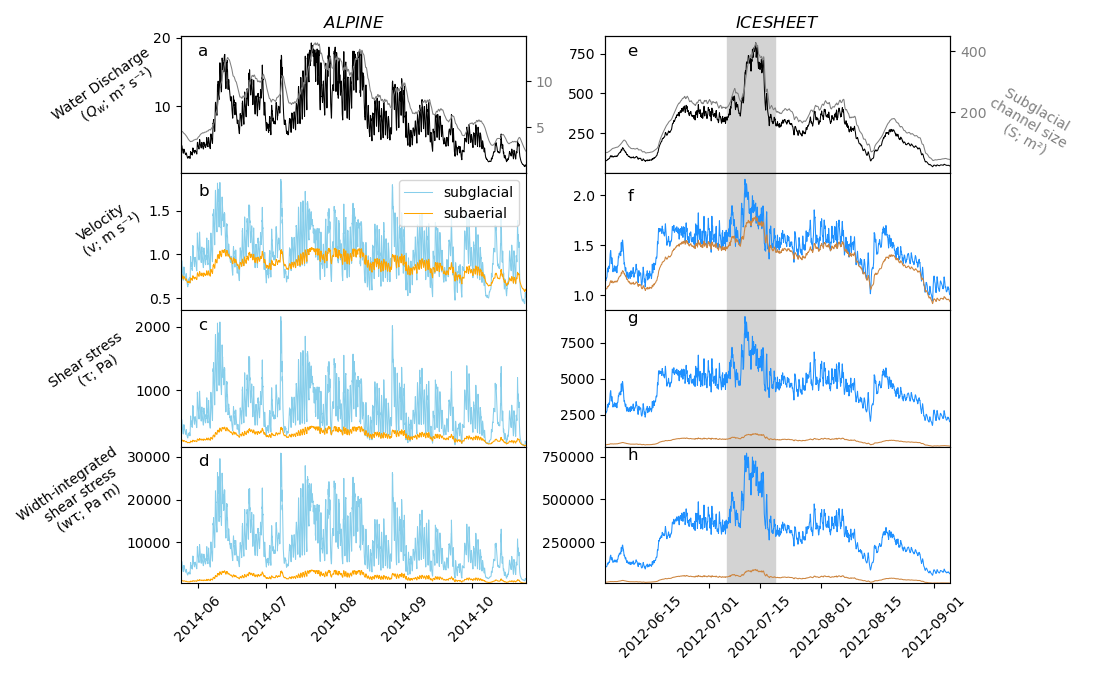
\includegraphics[width=0.7\linewidth]{Fig5_1hr.png}
    \caption{As Figure 5, with $1$ \,\unit{hr} aggregation.}
    \label{fig:model_outs_1hr}
  \end{figure}
\end{center}


\begin{center}
  \begin{figure}[h]
    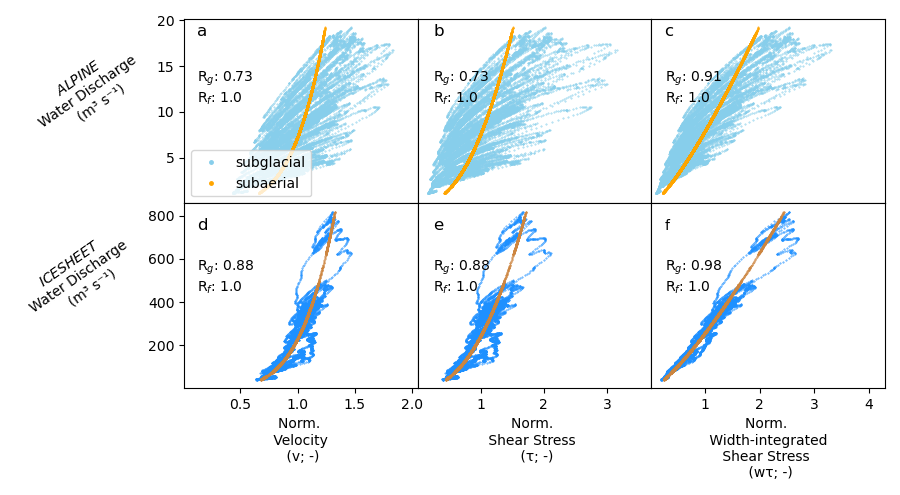
\includegraphics[width=0.7\linewidth]{Fig6_1hr.png}
    \caption{As Figure 6, with $1$ \,\unit{hr} aggregation.}
    \label{fig:Qw_vari_1hr}
  \end{figure}
\end{center}

\begin{center}
  \begin{figure}[h]
    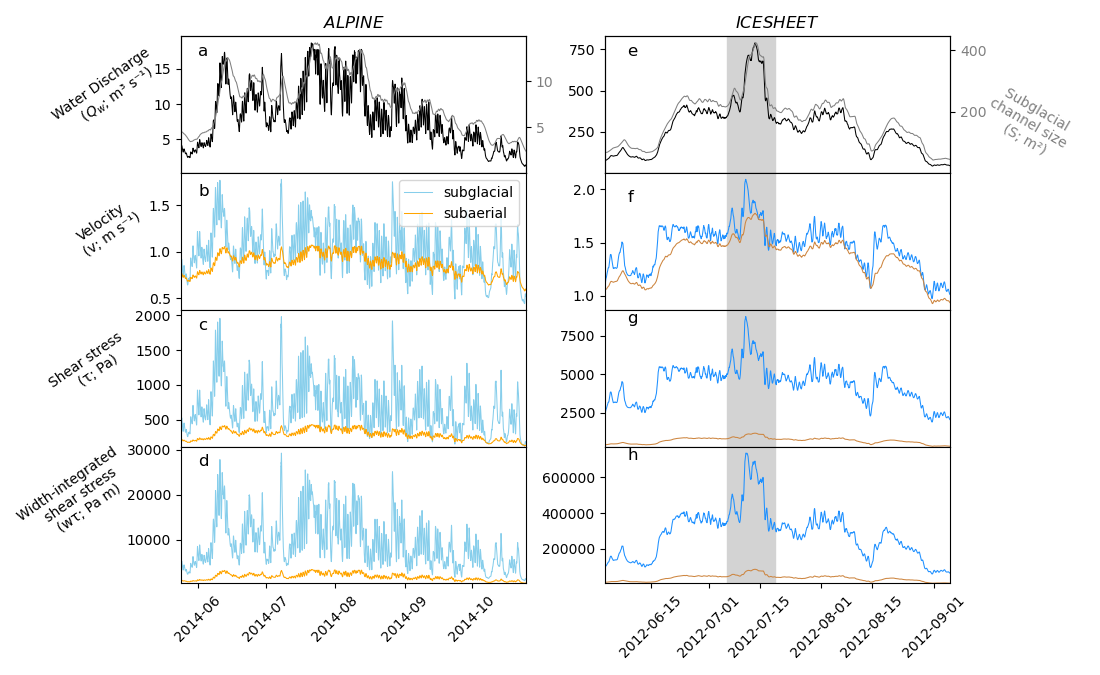
\includegraphics[width=0.7\linewidth]{Fig5_6hr.png}
    \caption{As Figure 5, with $6$ \,\unit{hr} aggregation.}
    \label{fig:model_outs_6hr}
  \end{figure}
\end{center}


\begin{center}
  \begin{figure}[h]
    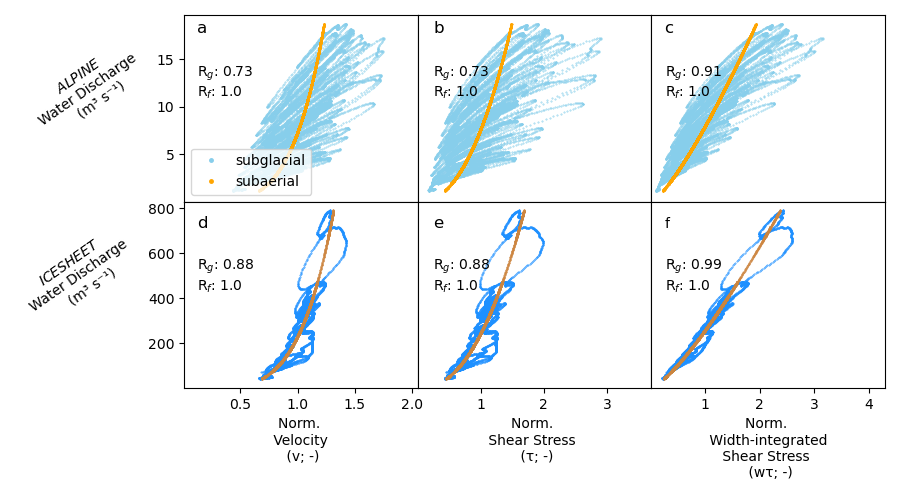
\includegraphics[width=0.7\linewidth]{Fig6_6hr.png}
    \caption{As Figure 6, with $6$ \,\unit{hr} aggregation.}
    \label{fig:Qw_vari_6hr}
  \end{figure}
\end{center}

\begin{center}
  \begin{figure}[h]
    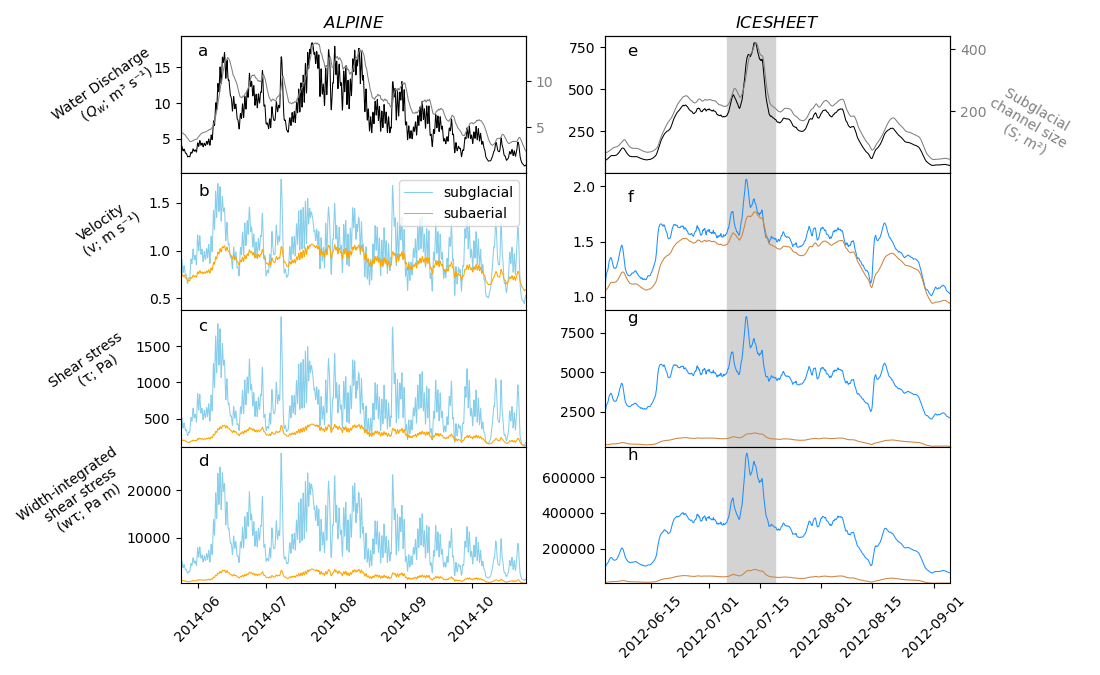
\includegraphics[width=0.7\linewidth]{Fig5_12hr.png}
    \caption{As Figure 5, with $12$ \,\unit{hr} aggregation.}
    \label{fig:model_outs_12hr}
  \end{figure}
\end{center}


\begin{center}
  \begin{figure}[h]
    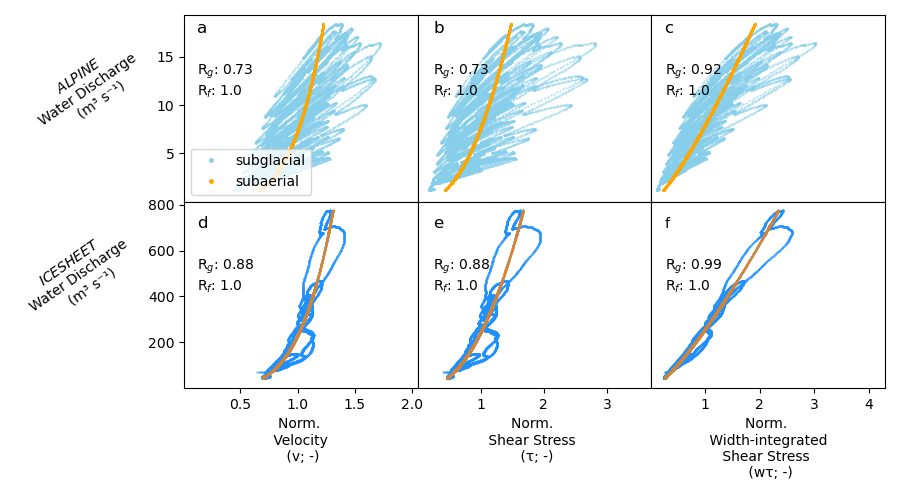
\includegraphics[width=0.7\linewidth]{Fig6_12hr.png}
    \caption{As Figure 6, with $12$ \,\unit{hr} aggregation.}
    \label{fig:Qw_vari_12hr}
  \end{figure}
\end{center}

\begin{center}
  \begin{figure}[h]
    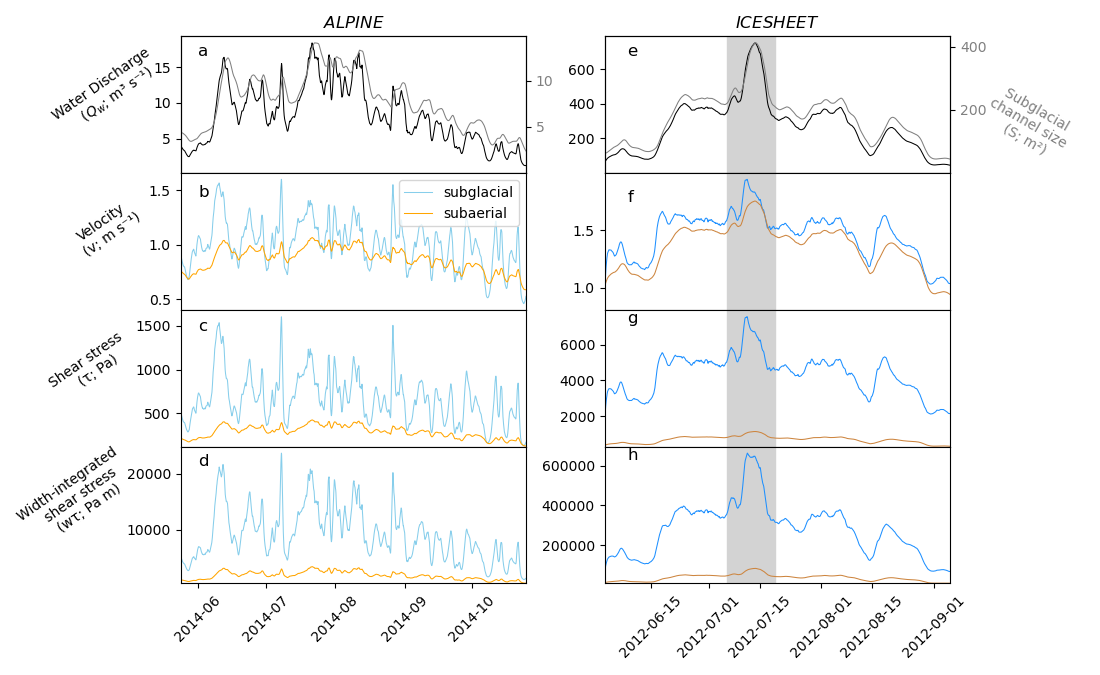
\includegraphics[width=0.7\linewidth]{Fig5_1day.png}
    \caption{As Figure 5, with $1$ \,\unit{day} aggregation.}
    \label{fig:model_outs_1day}
  \end{figure}
\end{center}


\begin{center}
  \begin{figure}[h]
    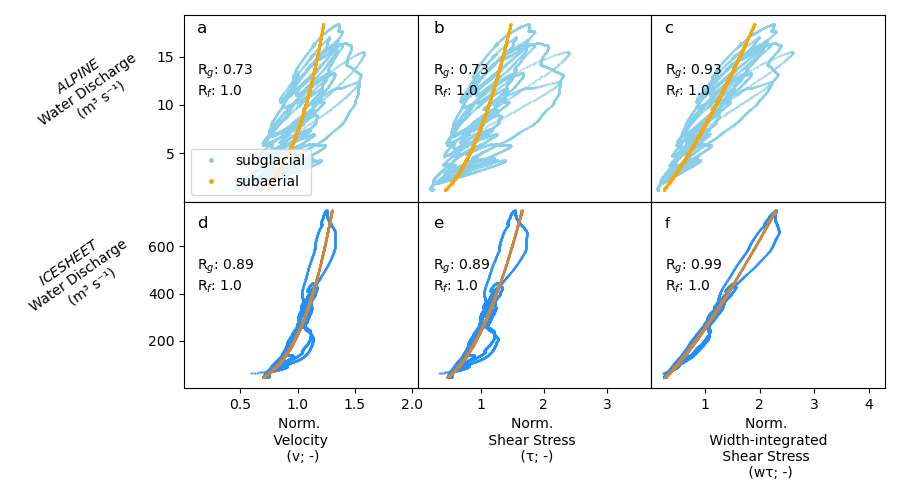
\includegraphics[width=0.7\linewidth]{Fig6_1day.png}
    \caption{As Figure 6, with $1$ \,\unit{day} aggregation.}
    \label{fig:Qw_vari_1day}
  \end{figure}
\end{center}

\begin{center}
  \begin{figure}[h]
    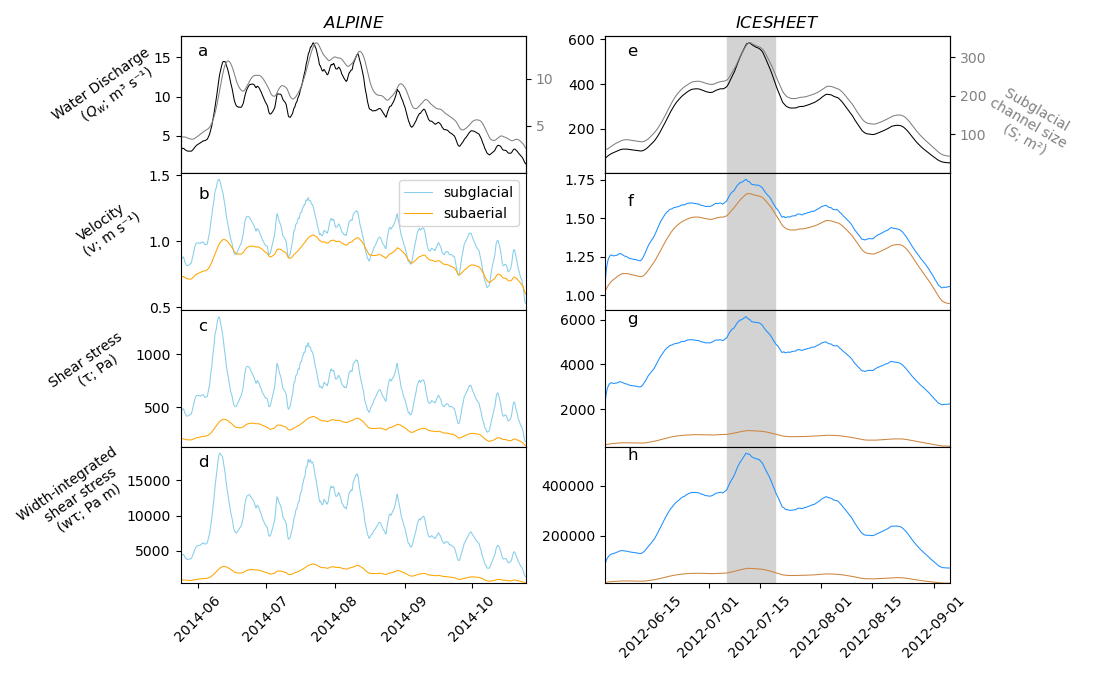
\includegraphics[width=0.7\linewidth]{Fig5_5day.png}
    \caption{As Figure 5, with $5$ \,\unit{day} aggregation.}
    \label{fig:model_outs_5day}
  \end{figure}
\end{center}




\begin{center}
  \begin{figure}[h]
    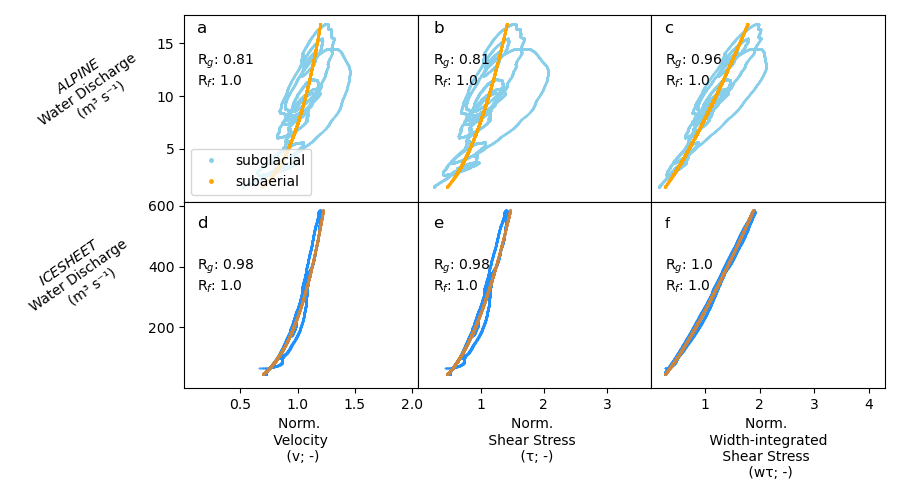
\includegraphics[width=0.7\linewidth]{Fig6_5day.png}
    \caption{As Figure 6, with $5$ \,\unit{day} aggregation.}
    \label{fig:Qw_vari_5day}
  \end{figure}
\end{center}

\begin{center}
  \begin{figure}[h]
    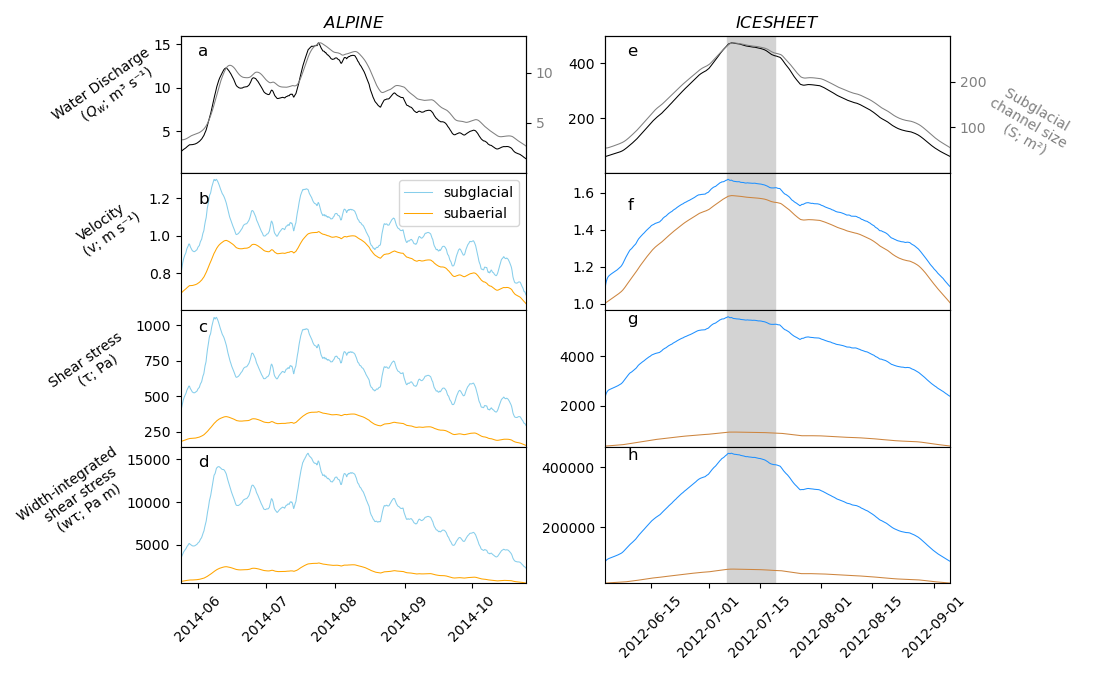
\includegraphics[width=0.7\linewidth]{Fig5_10day.png}
    \caption{As Figure 5, with $10$ \,\unit{day} aggregation.}
    \label{fig:model_outs_10day}
  \end{figure}
\end{center}


\begin{center}
  \begin{figure}[h]
    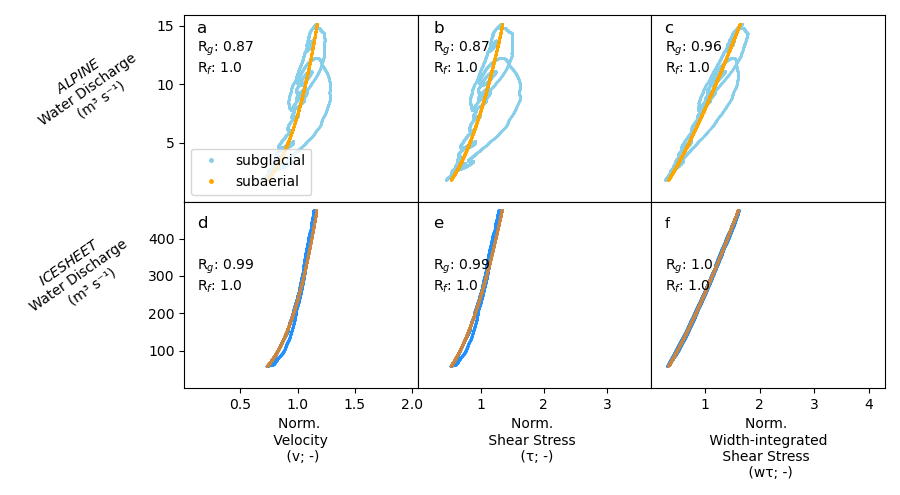
\includegraphics[width=0.7\linewidth]{Fig6_10day.png}
    \caption{As Figure 6, with $10$ \,\unit{day} aggregation.}
    \label{fig:Qw_vari_10day}
  \end{figure}
\end{center}

\begin{center}
  \begin{figure}[h]
    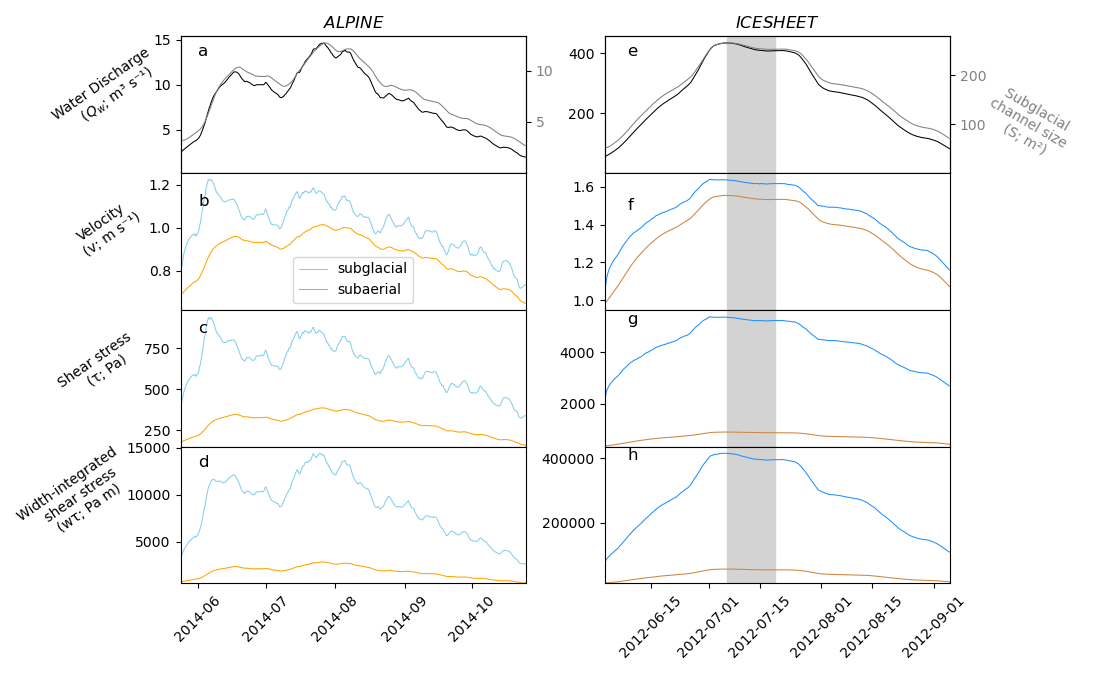
\includegraphics[width=0.7\linewidth]{Fig5_15day.png}
    \caption{As Figure 5, with $15$ \,\unit{day} aggregation.}
    \label{fig:model_outs_15day}
  \end{figure}
\end{center}


\begin{center}
  \begin{figure}[h]
    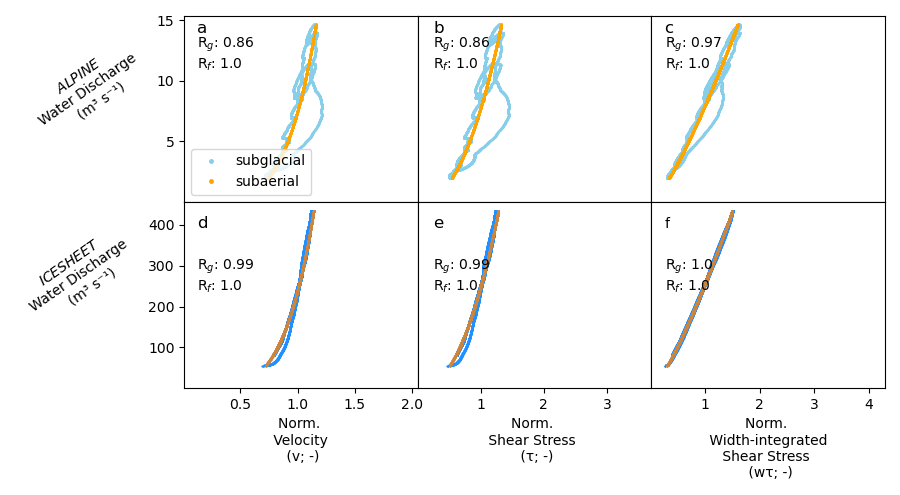
\includegraphics[width=0.7\linewidth]{Fig6_15day.png}
    \caption{As Figure 6, with $15$ \,\unit{day} aggregation.}
    \label{fig:Qw_vari_15day}
  \end{figure}
\end{center}



\begin{center}
  \begin{figure}[h]
    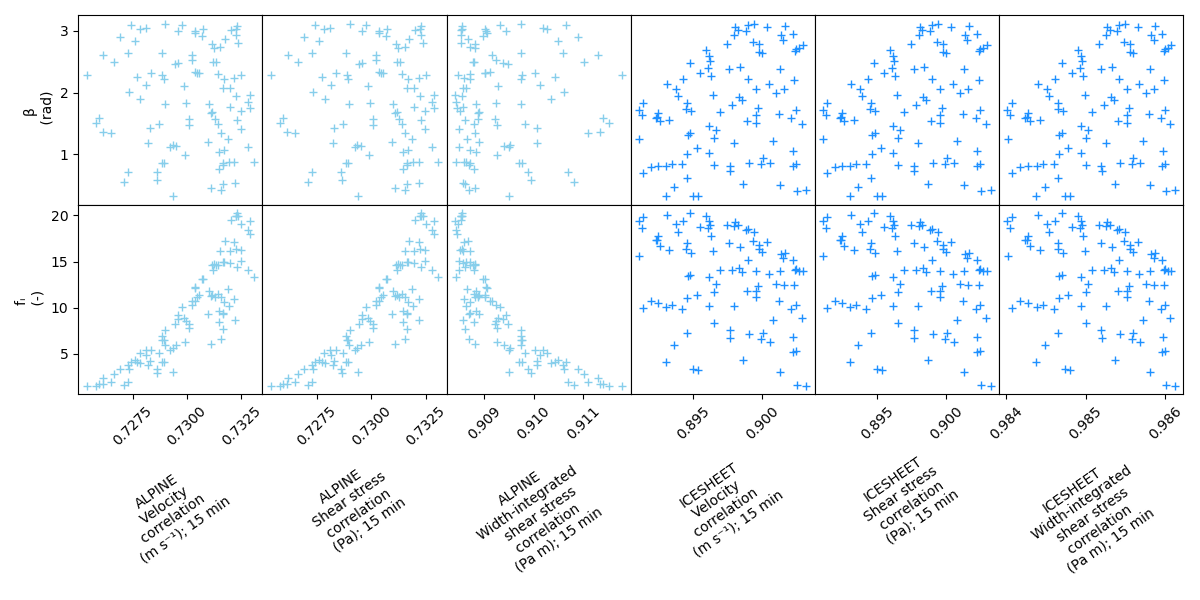
\includegraphics[width=0.7\linewidth]{FigS15.png}
    \caption{Parameter values of from ensemble run (Section 4.2) against rank correlation. Results show that across the parameter space, subglacial parameters do not reach a similar rank correlation of subaerial channels.}
    \label{fig:ensemble_vari}
  \end{figure}
\end{center}

\bibliographystyle{copernicus}
\bibliography{Paperlib.bib}
\end{document}

%% REFERENCES

%% The reference list is compiled as follows:

% \begin{thebibliography}{}

% \bibitem[AUTHOR(YEAR)]{LABEL1}
% REFERENCE 1

% \bibitem[AUTHOR(YEAR)]{LABEL2}
% REFERENCE 2

% \end{thebibliography}

%% Since the Copernicus LaTeX package includes the BibTeX style file copernicus.bst,
%% authors experienced with BibTeX only have to include the following two lines:
%%
%% 
%% \bibliography{example.bib}
%%
%% URLs and DOIs can be entered in your BibTeX file as:
%%
%% URL = {http://www.xyz.org/~jones/idx_g.htm}
%% DOI = {10.5194/xyz}


%% LITERATURE CITATIONS
%%
%% command                        & example result
%% \citet{jones90}|               & Jones et al. (1990)
%% \citep{jones90}|               & (Jones et al., 1990)
%% \citep{jones90,jones93}|       & (Jones et al., 1990, 1993)
%% \citep[p.~32]{jones90}|        & (Jones et al., 1990, p.~32)
%% \citep[e.g.,][]{jones90}|      & (e.g., Jones et al., 1990)
%% \citep[e.g.,][p.~32]{jones90}| & (e.g., Jones et al., 1990, p.~32)
%% \citeauthor{jones90}|          & Jones et al.
%% \citeyear{jones90}|            & 1990



%% FIGURES

%% When figures and tables are placed at the end of the MS (article in one-column style), please add \clearpage
%% between bibliography and first table and/or figure as well as between each table and/or figure.

% The figure files should be labelled correctly with Arabic numerals (e.g. fig01.jpg, fig02.png).


%% ONE-COLUMN FIGURES

%%f
%\begin{figure}[t]
%\includegraphics[width=8.3cm]{FILE NAME}
%\caption{TEXT}
%\end{figure}
%
%%% TWO-COLUMN FIGURES
%
%%f
%\begin{figure*}[t]
%\includegraphics[width=12cm]{FILE NAME}
%\caption{TEXT}
%\end{figure*}
%
%
%%% TABLES
%%%
%%% The different columns must be seperated with a & command and should
%%% end with \\ to identify the column brake.
%
%%% ONE-COLUMN TABLE
%
%%t
%\begin{table}[t]
%\caption{TEXT}
%\begin{tabular}{column = lcr}
%\tophline
%
%\middlehline
%
%\bottomhline
%\end{tabular}
%\belowtable{} % Table Footnotes
%\end{table}
%
%%% TWO-COLUMN TABLE
%
%%t
%\begin{table*}[t]
%\caption{TEXT}
%\begin{tabular}{column = lcr}
%\tophline
%
%\middlehline
%
%\bottomhline
%\end{tabular}
%\belowtable{} % Table Footnotes
%\end{table*}
%
%%% LANDSCAPE TABLE
%
%%t
%\begin{sidewaystable*}[t]
%\caption{TEXT}
%\begin{tabular}{column = lcr}
%\tophline
%
%\middlehline
%
%\bottomhline
%\end{tabular}
%\belowtable{} % Table Footnotes
%\end{sidewaystable*}
%
%
%%% MATHEMATICAL EXPRESSIONS
%
%%% All papers typeset by Copernicus Publications follow the math typesetting regulations
%%% given by the IUPAC Green Book (IUPAC: Quantities, Units and Symbols in Physical Chemistry,
%%% 2nd Edn., Blackwell Science, available at: http://old.iupac.org/publications/books/gbook/green_book_2ed.pdf, 1993).
%%%
%%% Physical quantities/variables are typeset in italic font (t for time, T for Temperature)
%%% Indices which are not defined are typeset in italic font (x, y, z, a, b, c)
%%% Items/objects which are defined are typeset in roman font (Car A, Car B)
%%% Descriptions/specifications which are defined by itself are typeset in roman font (abs, rel, ref, tot, net, ice)
%%% Abbreviations from 2 letters are typeset in roman font (RH, LAI)
%%% Vectors are identified in bold italic font using \vec{x}
%%% Matrices are identified in bold roman font
%%% Multiplication signs are typeset using the LaTeX commands \times (for vector products, grids, and exponential notations) or \cdot
%%% The character * should not be applied as mutliplication sign
%
%
%%% EQUATIONS
%
%%% Single-row equation
%
%\begin{equation}
%
%\end{equation}
%
%%% Multiline equation
%
%\begin{align}
%& 3 + 5 = 8\\
%& 3 + 5 = 8\\
%& 3 + 5 = 8
%\end{align}
%
%
%%% MATRICES
%
%\begin{matrix}
%x & y & z\\
%x & y & z\\
%x & y & z\\
%\end{matrix}
%
%
%%% ALGORITHM
%
%\begin{algorithm}
%\caption{...}
%\label{a1}
%\begin{algorithmic}
%...
%\end{algorithmic}
%\end{algorithm}
%
%
%%% CHEMICAL FORMULAS AND REACTIONS
%
%%% For formulas embedded in the text, please use \chem{}
%
%%% The reaction environment creates labels including the letter R, i.e. (R1), (R2), etc.
%
%\begin{reaction}
%%% \rightarrow should be used for normal (one-way) chemical reactions
%%% \rightleftharpoons should be used for equilibria
%%% \leftrightarrow should be used for resonance structures
%\end{reaction}
%
%
%%% PHYSICAL UNITS
%%%
%%% Please use \unit{} and apply the exponential notation



